\title{Uso de técnicas baseadas no conhecimento e lógicas \emph{fuzzy}}
\subtitle{Predição de classes e atributos de solos}
\author{por Michele Duarte de Menezes}
\maketitle
\begin{wrapfigure}{l}{0.15\textwidth}
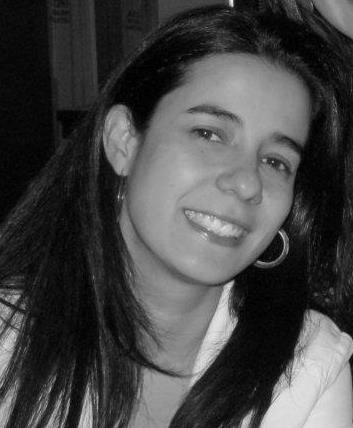
\includegraphics[width=0.15\textwidth]{figuras/foto-michele.png}
\end{wrapfigure}
Atualmente, diversas técnicas têm sido usadas para a predição de solos e seus atributos, algumas com a promessa de aumentar a acurácia, reduzir os custos e o tempo de execução. De um lado, temos as técnicas mais quantitativas ou pedométricas, onde a predição é baseada em técnicas estatísticas, geoestatísticas, mineração de dados ou de aprendizado de máquinas, e que, de modo geral, requerem um esquema amostral mais denso. Do outro lado, as técnicas baseadas no conhecimento, que buscam empregar efetivamente o conhecimento tácito (informações e técnicas adquiridas por experiência) na predição, com o intuito de reduzir algumas inconsistências e o custo dos mapeamentos manualmente confeccionados. Contudo, as técnicas pedométricas e as baseadas no conhecimento não são mutuamente exclusivas, e para ambas, o conhecimento das relações de solo-paisagem e prospecções de campo são necessários.\\
Hudson (1992), em seu consagrado artigo \emph{Soil Survey as Paradigm-based Science}, levantou que a maior parte do conhecimento a respeito de solos e paisagens encontra-se na forma de mapas de solos. Tal conhecimento, portanto, não é totalmente explícito aos demais usuários. E ainda, conforme levantado pelo Prof. Marcos Bacis Ceddia (UFRRJ) em sua palestra no Congresso Brasileiro de Ciência do Solo (2013), que abordou a respeito do mapeamento digital de solos - ou, conforme suas palavras, o mapeamento de solos no nosso tempo - se Dokuchaev estivesse vivo, quais ferramentas ele utilizaria para mapeamento? Será que o conhecimento já obtido, tanto tácito como em forma de mapas seriam ignorados?\\
Diante de tais técnicas, apontamentos e questões, apresento-lhes dois \emph{softwares} que fornecem um conjunto de ferramentas aos pedólogos para formalizarem as relações de solo-paisagem a partir de seus conhecimentos, de um modo mais quantitativo. O SoLIM (\emph{Soil Land Inference Model}) e o ArcSIE (\emph{Soil Inference Engine}) foram criados com o intuito de melhorar os métodos, a eficiência e a acurácia dos mapeamentos. O SoLIM é um software livre, já o ArcSIE é uma extensão do ArcGIS, mas é possível fazer o seu download gratuitamente. Tais ferramentas empregam alguns componentes, como o conhecimento especialista (\emph{expert}), a lógica \emph{fuzzy} ou nebulosa e vetores de similaridade.\\
Sistemas de conhecimento \emph{expert} buscam capturar o conhecimento tácito e integrá-lo em modelos de predição. Já a lógica \emph{fuzzy} configura-se como uma alternativa à lógica Booleana (modelo discreto, mapa do tipo polígono) no processo de inferência. A transição entre solos na paisagem se dá, frequentemente, de modo mais gradual e contínua, diferentemente das variações representadas por um mapa de polígono (Booleano). Existe certa incerteza na alocação dos limites entre os solos. Nesse sentido, a lógica \emph{fuzzy} busca representar a incerteza na predição, aplicando conceitos de verdade parcial, uma alternativa a rigidez subjetiva imposta aos solos.\\
Trazendo esses conceitos para uma aplicação mais real, a partir de covariáveis ambientais que representam os fatores de formação do solo em base SIG, e o ajuste de curvas de pertinência \emph{fuzzy}, as seguintes relações podem ser formalmente estabelecidas: em uma dada região fisiográfica, sabe-se que os Neossolos Litólicos ocorrem em faixas de altitude maiores que 850 m, cujo relevo é escarpado, a forma das vertentes são predominantemente côncavas e são formados a partir de granito-gnaisse. Uma vez que existe o conhecimento detalhado sobre as relações de solo paisagem da região, estabelecem-se curvas de pertinência \emph{fuzzy} para cada uma dessas instâncias, que consistem na base para a criação de mapas de pertinência \emph{fuzzy}. Um exemplo é dado para a declividade na \ref{fig:figura1}.\\
O conceito de pertinência ou pertencer a um grupo é modificado para incluir graus parciais de pertinência. O valor máximo de pertinência é geralmente 1 e representa o centro ou o conceito modal, e 0 representa não-pertinência (representados no eixo Y do gráfico). Valores entre 0 e 1 expressam diferentes graus de similaridade para o conceito central do tipo de solo. Conforme a curva ajustada (Figura 1), quanto maior a declividade (eixo X), maior o valor de pertinência (mais próximo de 1). Mais especificamente para o Neossolo Litólico e a declividade, ajusta-se o valor de 75 para o \emph{low unity} (relevo escapado apresenta declives maiores que 75\%, o que representa o valor ideal para ocorrência de Neossolos Litólicos, com valores de pertinência aumentando conforme aumenta a declividade), ajusta-se o valor de 45\% para o \emph{low cross} (valor que representa 50\% de pertinência \emph{fuzzy}).\\
\begin{figure*}[tb!]
\begin{minipage}[t]{1\linewidth}
\begin{center}
 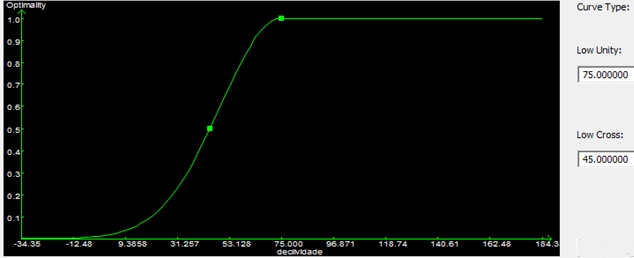
\includegraphics[width=\textwidth]{figuras/figura1.png}
 \caption{\emph{Layout} do SoLIM para o ajuste de curvas de pertinência \emph{fuzzy}.}
 \label{fig:figura1}
\end{center}
\end{minipage}
\end{figure*}
O próximo passo consiste na geração do mapa de pertinência \emph{fuzzy} a partir da curva gerada para a declividade, conforme apresentado na \ref{fig:figura2}. Quanto mais similar o solo ao conceito central prescrito, maior o valor de pertinência \emph{fuzzy} (mais próximo a 100). Estes conceitos são aplicados pixel a pixel. Notem a natureza contínua da distribuição, que serão a base para a composição do mapa de solos (polígono) e atributos (contínuo). Curvas devem ser ajustadas para as outras covariáveis, contemplando todas as instâncias e as diferentes classes de solos da área.\\
\begin{figure*}[tb!]
\begin{minipage}[t]{1\linewidth}
\begin{center}
   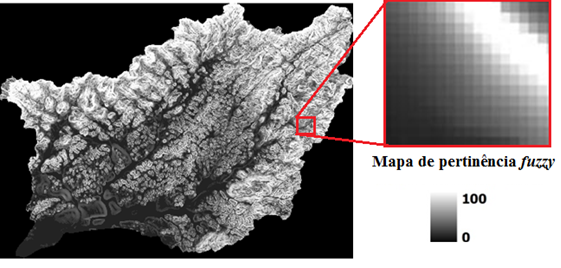
\includegraphics[width=\textwidth]{figuras/figura2.png}
   \caption{Mapa de pertinência \emph{fuzzy} gerado a partir do mapa de declividade.}
   \label{fig:figura2}
\end{center}
\end{minipage}
\end{figure*}
Para criar o mapa do tipo polígono, o ArcSIE ou SoLIM classificam pixel a pixel com o valor mais elevado de pertinência \emph{fuzzy}, de acordo com vetores de similaridade. Conforme, a \ref{fig:figura3}, o pixel assinalado será classificado como Neossolo Litólico. Portanto, os valores de pertinência \emph{fuzzy} foram usados para medir a incerteza associada ao processo de ``endurecimento'' (\emph{hardened}) ou defuzzificação do solo local, para gerar o mapa do tipo polígono.\\
E ainda, a partir das curvas estabelecidas e os mapas de pertinência \emph{fuzzy}, é possível a predição de atributos do solo de modo mais contínuo, a partir de apenas um valor típico, ou seja, um valor que melhor represente o conceito central ou modal de cada tipo de solo para a sua predição píxel a píxel na paisagem.\\
Eu comentei aqui apenas alguns pontos chave do processo de inferência. Detalhes sobre a matemática, os tipos de curvas ajustadas, bem como a estruturação das instâncias podem ser encontradas nos tutoriais dos softwares. Tanto o ajuste de curvas como a escolha dos valores típicos, tornam explícitos todos os detalhes da modelagem de solos e atributos, tornando-os assim potencialmente aplicáveis para outras regiões cujas relações de solo-paisagem são semelhantes. Acredito que seja esse um dos motivos para os autores considerarem tais ferramentas como promissoras para o mapeamento em massa, de modo mais rápido e com um menor custo.\\
\begin{figure}[htbp]
   \centering
   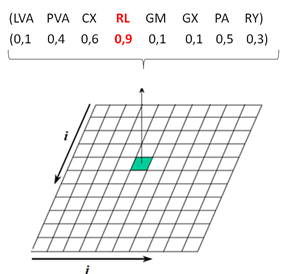
\includegraphics[scale=0.8]{figuras/figura3.png}
   \caption{Figure 3. Modelos de similaridade para representar informação espacial de solos.}
   \label{fig:figura3}
\end{figure}
Outra ferramenta interessante é o \emph{knowledge miner} (mineração do conhecimento), presente no SoLIM. Sob a premissa de que os mapas de solo representam a estrutura mental do pedólogo a respeito das relações de solo-paisagem, o usuário pode extrair informações de mapas pré-existentes por meio de curvas de frequência relativa, a partir de mapas derivados do terreno para cada polígono ou unidades de mapeamento. São computadas distribuições univariadas baseadas na estimação não-paramétrica de kernel. As curvas de frequência permitem descobrir o conhecimento \emph{expert} empregado. Nos Estados Unidos, esta ferramenta tem sido empregada para atualizar os mapas de solos já existentes, permitindo também detectar inconsistências. No Brasil, uma potencial aplicação desta ferramenta está na extração das curvas de frequência relativa em áreas de referência que possuem levantamentos de solos, e sua transferência para outras sem levantamento, mas com similaridade em termos de fatores de formação dos solos. 
Levantamentos de solos em escalas mais detalhadas são ainda necessários. Eis uma ferramenta promissora para aumentar a expressão geográfica de áreas mapeadas, com um menor custo.\\
Conforme levantado por alguns dos criadores do SoLIM (Shi et al., 2009 - \emph{Integrating Different Types of Knowledge for Digital Soil Mapping}), a aceitação de uma ferramenta é de suma importância: o usuário deve acreditar no sistema, e esta confiança é geralmente baseada no entendimento do usuário sobre o sistema. Os autores apontam também para uma maior aceitação desta ferramenta por parte dos pedólogos devido ao fato da abordagem ser baseada no conhecimento. De fato, tenho percebido também uma boa aceitação entre os mapeadores de solos os quais já comentei ou foram apresentados a ferramenta.\\
Pessoalmente, tive oportunidade de utilizar tais ferramentas durante o meu doutorado. Fui orientada pelo Prof. Nilton Curi (UFLA), um grande pedólogo que possui vasto conhecimento das relações de solo-paisagem das regiões em que desenvolvemos trabalhos. Fui orientada também pelo Prof. Phillip Owens (\emph{Purdue University}), cuja linha de pesquisa está um pouco mais relacionada ao mapeamento digital. A integração de tais conhecimentos, bem como o uso das ferramentas, me permitiu compreender, sedimentar e formalizar as relações de solo-paisagem de um modo mais quantitativo. Durante este período, lembrei-me de quando estava aprendendo a ler em minha infância. Para mim, era inevitável ler tudo ao meu redor a todo tempo: anúncios pelas ruas, jornais, revistas, televisão, etc. Do mesmo modo, quando comecei a aprender um pouco mais sobre a lógica \emph{fuzzy}, foi inevitável tentar ``encaixar'' ou ``ler'' os solos e outros fenômenos da natureza sob a ótica da lógica \emph{fuzzy}.\\
Já com relação às ferramentas propriamente ditas, quando comecei a usá-las faltavam alguns detalhes nos tutoriais, o que me fez gastar um tempo elevado com pequenos detalhes durante a modelagem. No entanto, os tutoriais foram muito melhorados desde então, e muitos artigos já foram publicados. Contudo, acho que o aprendizado da modelagem de solos por meio do ArcSIE ou SoLIM chega até ser um pouco intuitivo, o que é mais ou menos semelhante ao processo de mapeamento de solos.\\
O grande desafio, principalmente para esta técnica embasada no conhecimento, está na leitura da paisagem, no resgate da Geomorfologia, na aplicação adequada da Geomorfometria, e o afinamento com os conceitos da Pedologia. Isso se faz necessário pois os mapas de hoje requerem não apenas um \emph{layout} bonito, com cores atrativas, mas uma acurácia adequada, com a quantificação das incertezas, e geração de produtos para atender efetivamente as necessidades da sociedade. As atividades de campo são cruciais. Atrelar estas ferramentas à técnicas de mineração de dados podem ainda trazer informações relevantes à modelagem.\\
Existem ainda muitas áreas a serem mapeadas, e muito a ser testado com relação as ferramentas. Encorajo os interessados em mapeamento digital a aventurarem-se pelos tutoriais gratuitamente disponíveis na internet, que contém ainda uma base de dados para uma primeira familiarização.\\
\\
Link dos softwares para donwload:\\
SoLIM: \url{http://solim.geography.wisc.edu/about/index.htm}\\
ArcSIE: \url{http://www.arcsie.com/}\\
\\
\address{Michele Duarte de Menezes\\
  Universidade Federal Rural do Rio de Janeiro\\
  \email{michele\_duarte@ig.com.br}}

%%% Local Variables: 
%%% mode: latex
%%% TeX-master: documento-principal.tex
%%% End: 

